\chapter{Methodology}

\section{Datasets}
\subsection{SEN12-MS}
This thesis relies exclusively on the SEN12MS dataset~\cite{sen12ms_2019}, curated by Schmitt et al.. SEN12MS is a large-scale, globally distributed benchmark explicitly designed to advance research in multimodal Earth observation and deep learning. It comprises 180,662 georeferenced image triplets, each consisting of (i) dual-polarized Sentinel-1 synthetic aperture radar (SAR) data in VV and VH polarization ($\sigma^{0}$ backscatter values in decibel scale), (ii) full Sentinel-2 multispectral imagery spanning all 13 bands, and (iii) MODIS land cover maps derived from the MCD12Q1 product and resampled to 10 m resolution. Each triplet is stored as a 256 × 256 pixel GeoTIFF at 10 m ground sampling distance, corresponding to a spatial coverage of approximately 2.56 × 2.56 km per patch.

The Sentinel-1 component originates from ground-range-detected (GRD) products acquired in interferometric wide swath (IW) mode. These data were radiometrically calibrated and orthorectified against SRTM or ASTER digital elevation models to ensure accurate geolocation. The Sentinel-2 imagery was curated using a cloud-free mosaicking workflow on Google Earth Engine: within each region of interest (ROI), multiple observations collected during a given meteorological season of 2017 were composited such that cloud-contaminated pixels were systematically excluded. This procedure ensured that every ROI is represented by seasonally consistent, nearly cloud-free multispectral data. Finally, the MODIS land cover maps were used to generate categorical reference layers; however, due to their relatively coarse native resolution (500 m), they are subject to spatial inaccuracies even after upsampling.

\begin{figure}[htbp]
    \centering
    % First row: SAR images
    \begin{subfigure}{0.18\textwidth}
        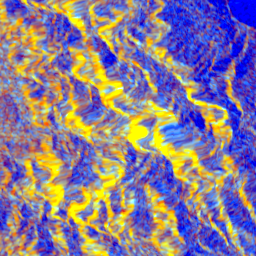
\includegraphics[width=\linewidth]{img/ROIs2017_winter_s1_68_p100.png}
    \end{subfigure}
    \begin{subfigure}{0.18\textwidth}
        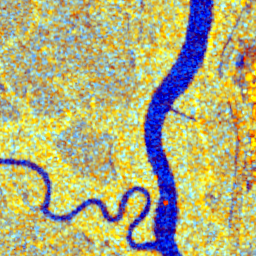
\includegraphics[width=\linewidth]{img/ROIs1970_fall_s1_105_p100.png}
    \end{subfigure}
    \begin{subfigure}{0.18\textwidth}
        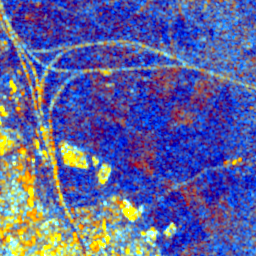
\includegraphics[width=\linewidth]{img/ROIs1970_fall_s1_128_p100.png}
    \end{subfigure}
    \begin{subfigure}{0.18\textwidth}
        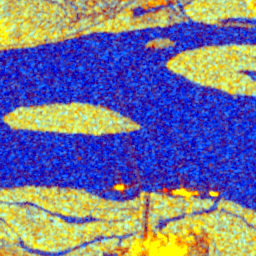
\includegraphics[width=\linewidth]{img/ROIs2017_winter_s1_104_p101.png}
    \end{subfigure}
    \begin{subfigure}{0.18\textwidth}
        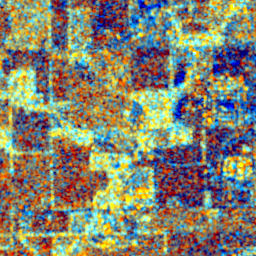
\includegraphics[width=\linewidth]{img/ROIs1970_fall_s1_145_p100.png}
    \end{subfigure}

    \begin{subfigure}{0.18\textwidth}
        \centering
        {\footnotesize \textit{Winter ROI-68-100}}
    \end{subfigure}
    \begin{subfigure}{0.18\textwidth}
        \centering
        {\footnotesize \textit{Fall ROI-105-100}}
    \end{subfigure}
    \begin{subfigure}{0.18\textwidth}
        \centering
        {\footnotesize \textit{Fall ROI-128-100}}
    \end{subfigure}
    \begin{subfigure}{0.18\textwidth}
        \centering
        {\footnotesize \textit{Winter ROI-104-101}}
    \end{subfigure}
    \begin{subfigure}{0.18\textwidth}
        \centering
        {\footnotesize \textit{Fall ROI-145-100}}
    \end{subfigure}
    
    \vspace{0.5em}

    % Second row: MS images
    \begin{subfigure}{0.18\textwidth}
        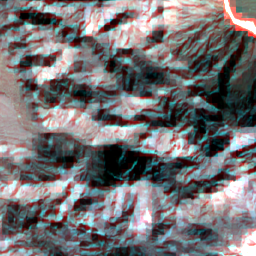
\includegraphics[width=\linewidth]{img/ROIs2017_winter_s2_68_p100.png}
    \end{subfigure}
    \begin{subfigure}{0.18\textwidth}
        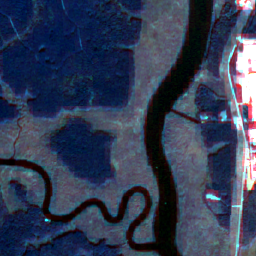
\includegraphics[width=\linewidth]{img/ROIs1970_fall_s2_105_p100.png}
    \end{subfigure}
    \begin{subfigure}{0.18\textwidth}
        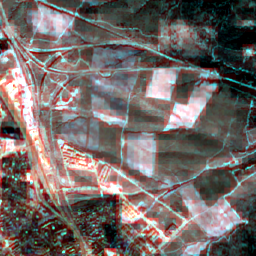
\includegraphics[width=\linewidth]{img/ROIs1970_fall_s2_128_p100.png}
    \end{subfigure}
    \begin{subfigure}{0.18\textwidth}
        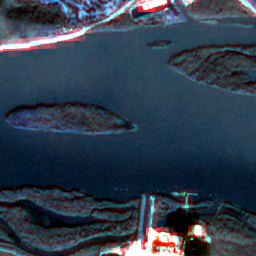
\includegraphics[width=\linewidth]{img/ROIs2017_winter_s2_104_p101.png}
    \end{subfigure}
    \begin{subfigure}{0.18\textwidth}
        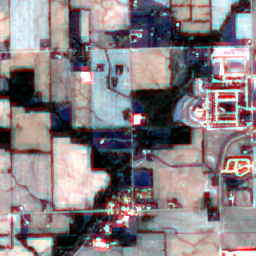
\includegraphics[width=\linewidth]{img/ROIs1970_fall_s2_145_p100.png}
    \end{subfigure}

    \caption{Sample pairs from the SEN12MS dataset. Top row: Sentinel-1 SAR patches (R: VV, G: VH, B: VV/VH). Bottom row: corresponding Sentinel-2 multispectral patches (only RGB bands).}
    \label{fig:sen12ms_pairs}
\end{figure}


Importantly, all triplets underwent manual verification by a remote sensing expert. This revision step ensured that each patch is free from major artifacts, severe registration errors, or residual cloud contamination, thereby guaranteeing the dataset’s quality and usability for machine learning tasks.

The ROIs were sampled globally across all inhabited continents and four meteorological seasons of 2017 to maximize spatial and temporal diversity. Nevertheless, it should be noted that the ROI selection was not purely random. In practice, locations were chosen to avoid large homogeneous areas such as deserts or oceans and to ensure inclusion of diverse land cover classes. While this design improves the dataset’s representativeness for a wide range of applications, it may introduce a bias toward heterogeneous landscapes and thus does not fully capture the true global distribution of land cover types.

For the purpose of this thesis, which addresses translation from SAR to multispectral optical imagery, only the Sentinel-1 and Sentinel-2 modalities are employed. The MODIS land cover products included in SEN12MS are disregarded, as they are not directly relevant to the translation task.

\subsection{SEN12 datasets Family}
SEN12MS is part of a broader line of datasets developed to foster multimodal remote sensing research. Its direct predecessor, SEN1-2~\cite{sen12_2018}, curated by the same research group, contained approximately 282,000 paired patches of Sentinel-1 VV data and Sentinel-2 RGB composites. While groundbreaking in bridging SAR and optical domains, SEN1-2 lacked georeferencing, full spectral coverage, and multi-polarization SAR, limiting its applicability for remote sensing research beyond proof-of-concept image translation.

SEN12MS addressed these limitations by introducing full multispectral coverage, dual-polarized SAR, geocoded products, and auxiliary land cover labels, making it a comprehensive multimodal benchmark. Building upon this foundation, the dataset family has since been extended. SEN12MS-CR~\cite{sen12ms-cr_2021} added temporally matched cloudy and cloud-free Sentinel-2 imagery alongside Sentinel-1 data, enabling the development and benchmarking of cloud removal methods under realistic atmospheric conditions. Subsequently, SEN12MS-CR-TS~\cite{sen12ms-cr-ts_2022} expanded the concept into the temporal domain, providing year-long multimodal time series with 30 co-registered Sentinel-1 and Sentinel-2 acquisitions per ROI. This evolution reflects a progression from simplified SAR–optical pairs, to globally diverse multimodal data, to temporally rich resources designed for time-series analysis and robust cloud removal.

A comparsion of these different datasets is provided in Table~\ref{tab:sen12_datasets}. In this thesis, however, the focus remains on the SEN12MS dataset, leveraging its multimodal SAR and multispectral imagery for the study of SAR-to-optical translation.

% in preamble:
% \usepackage{array,booktabs,adjustbox}
% ragged-right p-columns
\newcolumntype{P}[1]{>{\raggedright\arraybackslash}p{#1}}

\begin{table}[!h]
    \centering
    \caption{Comparison of datasets in the SEN12 family.}
    \label{tab:sen12_datasets}
    \setlength{\tabcolsep}{4pt} % tighter horizontal padding
    \renewcommand{\arraystretch}{1.15} % a bit more vertical room
    \begin{adjustbox}{max width=\textwidth, keepaspectratio=false}
    \begin{tabular}{P{2.6cm} P{3.4cm} P{3.4cm} P{3.6cm} P{3.6cm}}
        \toprule
        \textbf{Aspect} &
        \textbf{SEN1-2}~\cite{sen12_2018} &
        \textbf{SEN12MS}~\cite{sen12ms_2019} &
        \textbf{SEN12MS-CR}~\cite{sen12ms-cr_2021} &
        \textbf{SEN12MS-CR-TS}~\cite{sen12ms-cr-ts_2022} \\
        \midrule
        \textbf{Year released} &
        2018 & 2019 & 2021 & 2022 \\
        \addlinespace[6pt]
        \textbf{Main purpose} &
        Proof-of-concept SAR–optical translation &
        Multimodal learning and data fusion &
        Cloud removal with real cloudy/clear pairs &
        Multi-temporal cloud removal (sequence models) \\
        \addlinespace[6pt]
        \textbf{Modalities} &
        S1 (VV), S2 (RGB) &
        S1 (VV,VH), S2 (13 bands), MODIS LULC &
        S1 (VV,VH), S2 (13 bands; cloudy \& cloud-free) &
        S1 (VV,VH), S2 (13 bands; cloudy \& cloud-free time series) \\
        \addlinespace[6pt]
        \textbf{Georeferencing} &
        Not georeferenced &
        Fully georeferenced &
        Fully georeferenced &
        Fully georeferenced \\
        \addlinespace[6pt]
        \textbf{Spatial sampling} &
        Global patch pairs (282k) &
        180,662 patch triplets across 2017 seasons &
        169 ROIs; $>$100k patch triplets &
        53 ROIs; 30 time steps per ROI \\
        \addlinespace[6pt]
        \textbf{Temporal coverage} &
        Single time-point &
        Seasonal (2017) &
        Seasonal with paired cloudy/clear &
        Year-long time series (2018) \\
        \addlinespace[6pt]
        \textbf{Patch size} &
        $256\times256$ px &
        $256\times256$ px &
        $256\times256$ px &
        $256\times256$ px \\
        \addlinespace[6pt]
        \textbf{Notable limitations} &
        RGB only; VV only; no geocoding &
        MODIS labels are coarse (upsampled) &
        Mono-temporal pairs (no full time series) &
        Fewer ROIs; large storage ($\sim$2\,TB) \\
        \bottomrule
    \end{tabular}
    \end{adjustbox}
\end{table}


\section{Models}
\subsection{Pix2Pix Model}
The image translation task in this thesis is addressed using the \textit{pix2pix} framework, introduced by Isola et al.~\cite{pix2pix_2018}. Pix2pix is based on the concept of \textit{conditional generative adversarial networks} (cGANs), which extend the original GAN formulation by conditioning both the generator and discriminator on an input image. In this setup, the generator $G$ learns to map an input image $x$ to an output image $y$, while the discriminator $D$ learns to distinguish between real image pairs $\{x, y\}$ and synthesized pairs $\{x, G(x)\}$. This adversarial objective enforces that generated outputs are not only realistic but also structurally consistent with the given input.

Formally, the cGAN loss is defined as:
\begin{equation}
    \mathcal{L}_{cGAN}(G,D) = \mathbb{E}_{x,y}[\log D(x,y)] + \mathbb{E}_{x}[\log(1 - D(x,G(x)))].
\end{equation}
To encourage fidelity to the target image, the adversarial loss is combined with an $\ell_{1}$ reconstruction loss:
\begin{equation}
    \mathcal{L}_{\ell_1}(G) = \mathbb{E}_{x,y}[\|y - G(x)\|_1].
\end{equation}
The final objective is then:
\begin{equation}
    G^* = \arg \min_G \max_D \; \mathcal{L}_{cGAN}(G,D) + \lambda \mathcal{L}_{\ell_1}(G),
\end{equation}
where $\lambda$ balances realism and reconstruction accuracy. Following Isola et al., $\lambda = 100$ is typically used.

\paragraph{Generator architecture.}  
The generator is implemented as a \textit{U-Net} encoder–decoder~\cite{U-net_2015}. Unlike a plain encoder–decoder, U-Net introduces skip connections between corresponding downsampling and upsampling layers, allowing low-level spatial details from the input to directly propagate to the output. This design is particularly effective in tasks where the input and output share spatial structures, as in SAR-to-optical translation.

\paragraph{Discriminator architecture.}  
The discriminator follows a \textit{PatchGAN} design, which classifies local $N \times N$ patches of an image as real or fake instead of operating on the entire image~\cite{pix2pix_2018}. This approach emphasizes high-frequency correctness and enforces local realism, while the $\ell_1$ loss ensures global structural coherence. The original work demonstrates that a patch size of $70 \times 70$ provides a good trade-off between quality and efficiency.

\paragraph{Optimization.}  
Training alternates between updating $D$ to improve its ability to classify real versus fake pairs, and updating $G$ to fool $D$ while minimizing the $\ell_1$ distance to the target. The Adam optimizer~\cite{adam_optimizer_2017} with learning rate $2 \times 10^{-4}$ and momentum parameters $\beta_1=0.5$, $\beta_2=0.999$ is typically employed. Dropout is used at both training and inference time to introduce stochasticity, though in practice outputs remain largely deterministic.

\paragraph{Relevance to this work.}  
The pix2pix framework provides a principled and general-purpose solution for image-to-image translation tasks. In the context of this thesis, it is employed to learn mappings from Sentinel-1 SAR inputs to Sentinel-2 multispectral optical outputs. The combination of adversarial and reconstruction losses, together with the U-Net generator and PatchGAN discriminator, makes pix2pix particularly suitable for producing sharp, realistic, and structurally aligned multispectral predictions.


\section{Evaluation Metrics}
The effectiveness of SAR-to-optical image translation depends not only on the choice of translation models but also on the methods employed for quality assessment. Image Quality Assessment (IQA) serves two key purposes: (i) to objectively evaluate the quality of results produced by different models, and (ii) to guide the optimization of network architectures and algorithms~\cite{quality_assessment_S2OT}.

In~\cite{quality_assessment_S2OT}, five IQA metrics—SSIM, FSIM, MSE, LPIPS, and DISTS—were compared through image restoration experiments to identify suitable measures for SAR-to-optical translation. Their results showed that SSIM, MSE, and LPIPS consistently aligned with human perception, converged reliably, and effectively captured both structural and textural details, whereas FSIM often failed to capture fine details and DISTS exhibited instability. Consequently, SSIM, MSE, and LPIPS were recommended as complementary metrics for pixel-level fidelity, structural similarity, and perceptual quality. Nevertheless, as summarized in Table~\ref{tab:iqa}, SSIM, PSNR, and SAM remain the most widely used indicators in SAR-to-optical translation, fusion, and cloud removal tasks, while LPIPS and MSE appear far less frequently. This distribution is consistent with the findings reported in the literature survey~\cite{sar_2_opt_CGAN_survey_taxonomy}.

\textcolor{red}{TODO: specify which metrics will be used and why}

\begin{table}[h!]
\centering
\begin{tabular}{lll}
\toprule
\textbf{Metric} & \textbf{References} & \textbf{Frequency} \\
\midrule
Structural Similarity Index Measurement (SSIM)~\cite{iqa_ssim}
 & \cite{CR_Advances_Review_ORS, RS_Data_Fusion_GANs_sota, DiffCR, c_diffusion_s2o, s2o_ViT_cGAN, S2MS_GAN, c_guided_fus_s2ot, transfusion_cr, trans_gan_CF, hvt_cgan, msf_gan, diffusion_memory} 
 & 12 \\
Peak Signal-to-Noise Ratio (PSNR)~\cite{iqa_psnr}
 & \cite{CR_Advances_Review_ORS, DiffCR, CR_RS_spati_atten_GAN, s2o_ViT_cGAN, CR_RS_GAN_s2o, S2MS_GAN, c_guided_fus_s2ot, transfusion_cr, trans_gan_CF, hvt_cgan, msf_gan, diffusion_memory} 
 & 12 \\
Spectral Angle Mapper (SAM)~\cite{iqa_sam}
 & \cite{aCGAN_fuse_sar_MS, RS_Data_Fusion_GANs_sota, CR_RS_GAN_s2o, S2MS_GAN, c_guided_fus_s2ot, transfusion_cr, trans_gan_CF, cond_brownian, hvt_cgan, msf_gan} 
 & 11 \\
Fréchet Inception Distance (FID)~\cite{iqa_fid}
 & \cite{DiffCR, c_diffusion_s2o, s2o_ViT_cGAN, cond_brownian, hvt_cgan, msf_gan} 
 & 6 \\
Root Mean Square Error (RMSE) 
 & \cite{aCGAN_fuse_sar_MS, CR_Advances_Review_ORS, RS_Data_Fusion_GANs_sota, CR_RS_GAN_s2o, c_guided_fus_s2ot} 
 & 5 \\
Learned Perceptual Image Patch Similarity (LPIPS)~\cite{iqa_lpips}
 & \cite{CR_Advances_Review_ORS, DiffCR, S2MS_GAN, cond_brownian, diffusion_memory} 
 & 5 \\
Mean Absolute Error (MAE) 
 & \cite{CR_RS_GAN_s2o, c_guided_fus_s2ot} 
 & 2 \\
Mean Square Error (MSE) 
 & \cite{CR_RS_spati_atten_GAN, trans_gan_CF} 
 & 2 \\
\bottomrule
\end{tabular}
\caption{Common evaluation metrics for SAR-to-optical and cloud removal tasks.}
\label{tab:iqa}
\end{table}

\paragraph{SSIM}
The Structural Similarity Index (SSIM)~\cite{iqa_ssim} measures perceptual similarity by comparing local patterns of luminance, contrast, and structure between two images. Unlike pixel-wise errors, it models human visual sensitivity to structural distortions~\cite{DiffCR,hvt_cgan}, which is crucial for evaluating translated images. For two images $x$ and $y$, SSIM is defined as
\begin{equation}
\text{SSIM}(x,y) = \frac{(2\mu_x \mu_y + c_1)(2\sigma_{xy} + c_2)}{(\mu_x^2 + \mu_y^2 + c_1)(\sigma_x^2 + \sigma_y^2 + c_2)},
\end{equation}
where $\mu_x, \mu_y$ are means, $\sigma_x^2, \sigma_y^2$ variances, and $\sigma_{xy}$ the covariance. Values close to 1 indicate strong structural similarity. By focusing on local patterns of pixel intensities and their structural relationships, SSIM better reflects perceptual fidelity compared to raw pixel-difference metric


\paragraph{PSNR} 
The Peak Signal-to-Noise Ratio (PSNR) quantifies the distortion between a reconstructed image and its reference. PSNR is directly related to the Mean Squared Error (MSE), measuring pixel-level fidelity by comparing the residual error to the maximum possible signal intensity. For two images $x$ and $y$, PSNR is defined as
\begin{equation}
\text{PSNR}(x,y) = 10 \cdot \log_{10} \left( \frac{MAX^2}{\text{MSE}(x,y)} \right),
\end{equation}
with
\begin{equation}
\text{MSE}(x,y) = \frac{1}{N} \sum_{i=1}^{N} (x_i - y_i)^2,
\end{equation}
where $x_i$ and $y_i$ denote the pixel values of the generated and reference images, $N$ is the total number of pixels, and $MAX$ is the maximum pixel intensity (typically $255$ for 8-bit images).  

Higher PSNR values indicate lower distortion and better image quality, as they imply that the reconstructed image more closely approximates the reference. Despite its popularity for tasks such as denoising and compression, PSNR is limited by its purely pixel-wise formulation and often correlates weakly with human visual perception~\cite{DiffCR}.

\paragraph{SAM} 
The Spectral Angle Mapper (SAM), originally proposed by Kruse et al.~\cite{iqa_sam} in 1993, is widely employed in remote sensing to evaluate the spectral fidelity of reconstructed images. SAM regards the spectrum of each pixel as a high-dimensional vector and quantifies similarity by measuring the angle between the generated and reference spectral vectors. For two spectral vectors $x$ and $y$, SAM is defined as
\begin{equation}
\text{SAM}(x,y) = \arccos \left( \frac{\langle x, y \rangle}{\|x\|_2 \cdot \|y\|_2} \right),
\end{equation}
where $\langle x,y \rangle$ denotes the dot product and $\|\cdot\|_2$ is the Euclidean norm.  

SAM is typically expressed in degrees, with smaller values indicating higher spectral similarity and less distortion. Since it only considers the direction of the spectral vectors and not their magnitude, SAM is invariant to changes in illumination, making it particularly suitable for remote sensing and multispectral image analysis~\cite{S2MS_GAN}. In practice, the global SAM score is computed as the average angle across all pixels in the image.

\paragraph{LPIPS} 
The Learned Perceptual Image Patch Similarity (LPIPS) metric was proposed by Zhang et al.~\cite{iqa_lpips} to provide a perceptual measure of image similarity that better aligns with human visual judgment. It compares feature activations from pretrained convolutional networks, thereby capturing high-level semantics and perceptual realism. For two images $x$ and $y$, LPIPS is defined as
\begin{equation}
\text{LPIPS}(x,y) = \sum_{l} w_l \cdot \| f_l(x) - f_l(y) \|_2,
\end{equation}
where $f_l(\cdot)$ denotes the feature representation in the $l$-th layer of the network and $w_l$ is a learned weight.  

By measuring differences in a deep feature space rather than raw pixel intensities, LPIPS reflects perceptual similarity and visual realism. Lower LPIPS values indicate that the generated image is closer to the reference in terms of human-perceived quality~\cite{CR_Advances_Review_ORS,DiffCR}, making this metric particularly useful for evaluating the naturalness of translated images.

\paragraph{FID} 
Introduced in 2018 by Heusel at el.~\cite{iqa_fid}, the Fréchet Inception Distance (FID) is a perceptual metric that evaluates the realism of generated images at the distributional level. Instead of comparing images pixel by pixel, FID measures the distance between the feature distributions of generated and reference images, extracted by a pretrained Inception network. Let $(\mu_r, \Sigma_r)$ and $(\mu_g, \Sigma_g)$ denote the mean and covariance of the reference and generated feature distributions, respectively. FID is defined as
\begin{equation}
\text{FID} = \| \mu_r - \mu_g \|_2^2 + \text{Tr}\left( \Sigma_r + \Sigma_g - 2(\Sigma_r \Sigma_g)^{1/2} \right).
\end{equation}

Lower FID values indicate closer alignment between generated and real image distributions. While LPIPS assesses pairwise perceptual similarity, FID captures distributional alignment, making the two metrics complementary.


\paragraph{Evaluation Protocol}
The evaluation of SAR-to-optical translation performance was conducted using PSNR, SSIM, and SAM, complemented by a perceptual metric (LPIPS or FID). PSNR quantifies pixel-level fidelity, SSIM assesses local structural similarity, and SAM measures spectral consistency across all bands, which is critical in multispectral applications. To additionally capture perceptual realism beyond pixel-wise statistics, a deep feature–based perceptual score was employed, with LPIPS enabling pairwise comparisons and FID providing distributional similarity. For outputs with more than three bands, perceptual metrics were computed on a fixed RGB composite for both reference and prediction, and this limitation was explicitly acknowledged. This combination of metrics provides a comprehensive assessment covering spatial fidelity, structural integrity, spectral accuracy, and perceptual quality.

\begin{table}[h!]
	\centering
	\caption{Summary of evaluation metrics for SAR-to-multispectral translation.}
	\begin{tabularx}{\textwidth}{p{1.7cm}X X X}
		\toprule 
		\textbf{Metric} & \textbf{Aspect Evaluated} & \textbf{Advantages} & \textbf{Limitations} \\
		\midrule 
		PSNR  & Pixel-level fidelity via mean squared error ratio & Simple, widely used, interpretable in terms of noise/distortion & Correlates weakly with human perception; sensitive to pixel shifts \\
		SSIM  & Structural similarity (luminance, contrast, texture) & Captures perceptual structure better than PSNR; patch-based & Still intensity-based; limited correlation with perceptual realism \\
		SAM   & Spectral fidelity across bands & Invariant to illumination; critical for multispectral data integrity & Ignores spatial/structural context; only reflects spectral angle \\
		LPIPS & Perceptual similarity using deep features (pairwise) & Aligns well with human judgment; sensitive to high-level semantics & Requires pretrained CNN; limited to 3-channel inputs unless adapted \\
		FID   & Distributional similarity in feature space & Evaluates realism of entire image sets; widely adopted in generative models & Requires large sample size; sensitive to preprocessing; assumes Gaussian feature distributions \\
		\bottomrule
	\end{tabularx}
\end{table}
